現実世界において対面する多くのデータは離散的ではない。音声や映像は無論のこと、道程や時間も連続的なデータ(アナログデータ)である。アナログデータをそのままに記録・伝達することは多くの場合難しい。そのため、保存にあたっては復元可能なデジタルデータへと置き換えて保存される場合が多い。

本章では、まずアナログデータをそのまま連続的な量として記録できる例を説明する。次いで、デジタルデータへの置き換えについて、その手法と制約、影響等を論ずる。

\section{連続データの記録}

デジタルデータの保存方法がなかった頃、あるいは乏しかった頃、アナログデータは変換なしにそのまま保存されていた。図画はその最も原始的なものであろう。風光明媚な風景を伝えたいと描かれた風景画、その人物の偉大さを讃えた肖像画、建物の設計図などは、人間の視覚による差異や筆致の巧拙を別にすれば、おおよそそのままに伝えている。あるいは立像なども直接保存する一例と言えよう。

時代は下り、人はアナログのデータを直接に、あるいは必要に応じて媒体を変換させつつも連続性を保ったまま保存する術を開発してきた。ここでは、光・音・運動の3例を紹介する。

\subsection{光の保存例:写真}
光をそのまま保存している例としては写真がある。写真はカメラを用いて図\ref{fig2_1}に示すように光をフィルムに投影する。
\begin{figure}[htbp]
\centering
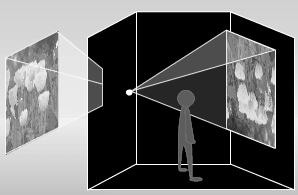
\includegraphics[width=0.6\linewidth,keepaspectratio,bb=0 0 298 195]{fig/fig2_1.png}
\caption{ピンホールカメラ。Canonサイトより引用}\label{fig2_1}
\end{figure}

フィルムには感光体があり、この感光体が受けた光に応じて変化を起こす。記録自体はこれで完了である。実際に読み出すには、この変化した感光体を薬品などに浸して化学変化させて再度発色させるなどの工程が行われる。一般には現像と呼ばれる工程である。

フィルムの化学変化を光によって起こすという方法で、そのままでは消えてしまう光を物質の際によって保存しているのが写真なのである。

\subsection{音の保存例:レコード}
音声・音楽の保存というのは非常に顕著な変化を見せている。戦後の頃には、レコードが主たる媒体であった。レコードは薄い板の両面に音楽のデータを刻む事ができる媒体だった。現代でも稀に"両A面シングル"などという呼び名があるが、これは元々レコードにA面とB面という区別があったことから出来た言葉である。

その後、ABがなくなり、CDへと移った(桂文珍「心中恋電脳」)。コンパクト・ディスクは片面のみにデジタルデータで保存を行い、これを光学的に読み取って音声へと変換することで音楽を鳴らし始めた。ここがアナログとデジタルの分かれ目である。AB…つまりレコードはアナログであったが、CDはデジタルということである。アナログとデジタルの変換をA/D変換などと書くことがあるが、なるほど、A(B)/(C)Dの変換と考えると確かにこの変化は顕著である。…洒落はともかく、このデジタルとなった音楽をインターネットを介して運ぶようになったのが現代のダウンロードによる音楽配信である。ことほど左様に音声・音楽データの保存は記録や通信の変化に対応しているのである。

レコードでの音楽の保存はアナログな音を「そのままに」保存しているのであるが、これは一体どういう原理であろうか。

音声というのは空気の振動である。この空気の振動を保存すれば良い…これがレコードの最も基本的な考えである。空気の振動を適当なもの(通常は針)に集音して伝え、下の面で回転している(記録前の)レコードに当てる。これにより、レコードが振動に合わせて削られる。再生するときは、逆にレコードの削れた面をなぞるように針をあて、この振動を増幅させて音声とする。

空気の振動ということでは動きもするし減衰もする。そのため、空気の振動をそのまま別の振動へと変換して保存するのがレコードという媒体の原理である。

\subsection{運動の保存例:地震計}
レコードは空気の振動であったが、同じ原理を用いて地面の振動=地震の揺れを記録するのが地震計である。

地震計は錘(おもり)に糸をつけた振り子を用意し、錘を不動点として地面の揺れを記録する。(図\ref{fig2_2})
\begin{figure}[htbp]
\centering
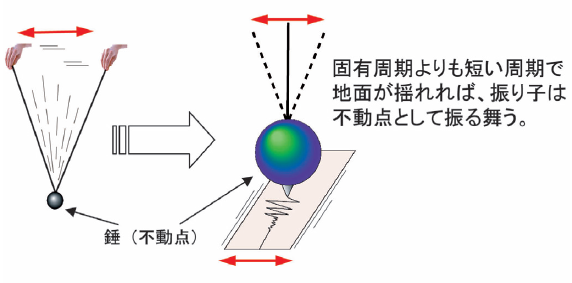
\includegraphics[width=0.6\linewidth,keepaspectratio,bb=0 0 572 283]{fig/fig2_2.png}
\caption{地震計の原理。札幌管区気象台サイトより引用}\label{fig2_2}
\end{figure}

振り子の糸の端を素早く左右に動かした場合、錘は動かない。そのため、錘の下にペンをつけ地面に紙を置くと紙だけが揺れるため地面の動きを記録することができる。これを複数の方向(東西・南北・上下)用意すれば、地震の3次元的な揺れをそのまま記録することができる。レコードと違い、これをそのままに再現するのは困難であるが(また、再現されると非常に迷惑でもあるが)、地震の状況を伝える資料として保存する、あるいは伝えるのには格好の方法と言えよう。


\section{デジタルデータへの変換}

アナログデータの保存の例を示してきたが、アナログデータは必ずしも移行や保存が楽ではなく、また通信の観点から見ても例えば地震計をそのままに伝送するには紙を運送する必要がある。また、レコードのように専用の機器が必要になる場合も多く、取扱が簡便であるとは言い難い。そこで、汎用性を持った記録・通信のためにデジタルデータへ変換して保存するということが考えられる。

アナログデータをデジタルデータに変換する場合というのは、連続性のあるものから代表値を選び出してそれを順に記録することとなる。これは、次の三つの手順からなる。
\begin{enumerate}
\item \textbf{標本化}\index{ひょうほんか@標本化}(Sampling):アナログデータから代表値(サンプリング値・標本値)を取得する。
\item \textbf{量子化}\index{りょうしか@量子化}(Quantization):サンプリング値をデジタルで表現可能な最も近い値へと丸める。
\item \textbf{符号化}\index{ふごうか@符号化}(Encoding):量子化された値(量子化値)を記録できる形式に変換する(多くはビット列となる)。デジタルデータの符号化と同様である。
\end{enumerate}

この途上において、最初に歴史に学んだ通り、取捨選択されている部分が存在する。アナログとデジタルを比較した文脈においては、しばしば「デジタルにはないアナログの良さ」が標榜されているが、その多くはこの標本化や量子化において捨象された部分を指す。捨象された部分というのは伝達に不都合であるとか影響が少ない、あるいはそもそも不必要といった部分であるため、伝達や記録と言った主目的を達するために、本質的でない部分を犠牲にしているというのがデジタルへの変換の基本的な考えである。これはそのまま、「微細な心情等は伝わりづらいが効率的」とされるデジタルデータと、「扱いは面倒だが機微が伝わる」とされるアナログデータの印象にも繋がっていると言えよう。

閑話休題。上記のようにデジタルデータへと変換し保存された後は、保存されたデータを読み取ってその値を適切につなぐことで原データの近似データを得られる。この近似データが十分良い近似であればアナログデータの保存という目的は達せられたと言える。では、この適切な近似データを得るためにはどうすればよいだろうか?以後、変換の各手順とともに良質な変換を担保する条件を見ていこう。

\section{アナログデータの標本化}

アナログデータの標本点を定め、標本値を取得するのがアナログデータの標本化である。つまり、連続的なデータの何点かを取り、その点の値を取得するという動作を標本化と呼ぶ(図\ref{fig2_3})。

\begin{figure}[htbp]
\centering
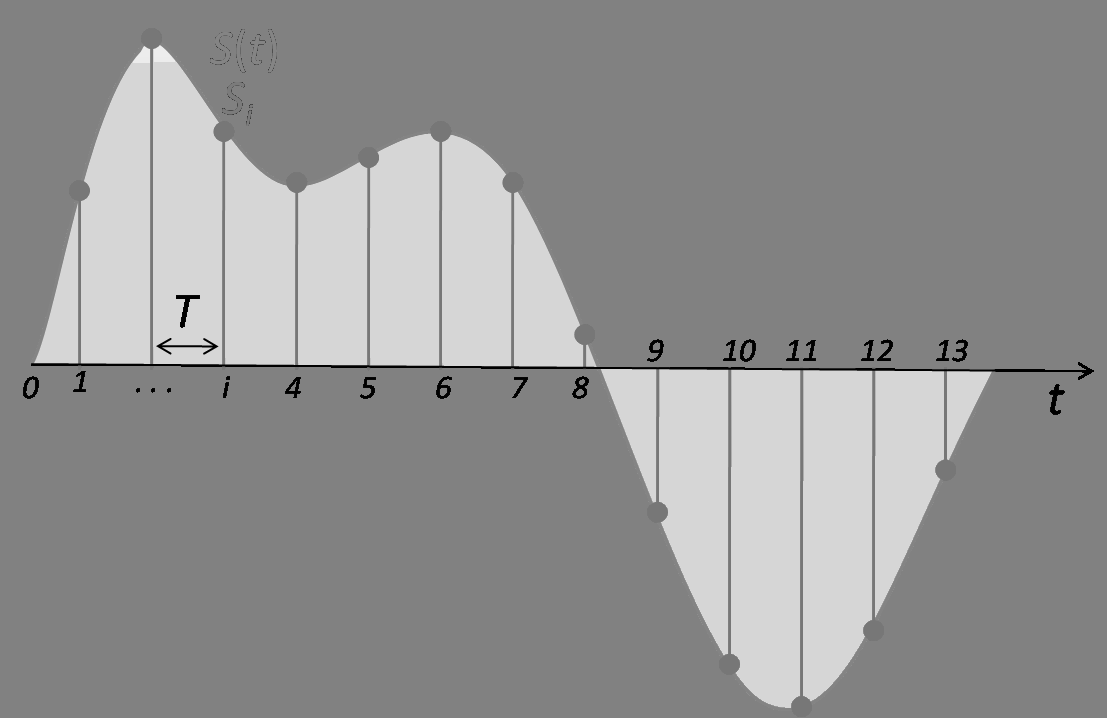
\includegraphics[width=0.6\linewidth,keepaspectratio,bb=0 0 1107 718]{fig/fig2_3.png}
\caption{標本化の例。各点における縦線が標本値を示す。Wikipediaより引用}\label{fig2_3}
\end{figure}

得られた標本値を適切に結ぶことができれば原データを復元できる。しかし、標本値が十分な個数なければ原データを正確に・精確に復元することは困難になるだろう。だからといって過剰に多くの点を取ってしまえばデータの量が嵩んでしまうのは目に見えている。これらの観点からすれば、原データを復元するに必要な最小限のデータを標本値として取得することが望ましい。では、どのようなデータをとれば原データを復元できるだろうか?その答えの源流は、19世紀初頭頃の物理学の話に遡る。

\subsection{Fourierの夢}

18世紀から19世紀にかけて活躍した、フランスの数学者・物理学者Jean Baptiste Joseph Fourier男爵は、ある物体中で熱がどのように伝わるのかを表す熱伝導方程式を導出した。もっとも、熱伝導方程式は方程式と言っても一般にいう代数方程式―未知数を含む関係式があり、限られた値しか認められないような等式―ではなく、関数方程式―未知の関数に関する関係式があり、これを満たす関数が限られる等式―である。つまり「あてはまる数値を求める方程式」ではなく「あてはまる関数を求める方程式」である。

Fourierは著書「熱の解析的理論」において、"任意の関数は、三角関数\footnote{ここでは$\sin,\cos$のこと。}の級数\footnote{無限和のこと。}で表すことができる"と主張した。Fourier自身が与えたこの主張に対する証明は不十分であったが、後世の数学者により「ほとんどあらゆる」関数について三角関数の総和形式で表されることが示された。方程式論や方程式の解法に終生興味を持ち続けたFourierの夢が花開いたといえる。このように、関数を三角関数の総和形式に表すことを、\textbf{Fourier展開}\index{Fourierてんかい@Fourier展開}あるいは\textbf{Fourier変換}\index{Fourierへんかん@Fourier変換}と呼ぶ\footnote{一般には、有限区間での総和をFourier展開、無限区間での総和をFourier変換と呼び分けている。}。

三角関数は周期的に変化する。このため、三角関数は波を表していると言える。波の周期の逆数を\textbf{周波数}\index{しゅうはすう@周波数}と呼ぶ。Fourier展開とは、異なる周波数の波を十分な個数集め、必要な程度に増幅あるいは減衰させて足し合わせることによって関数を表せるという主張である。各々の周波数における増幅あるいは減衰を表す係数を\textbf{周波数スペクトル}\index{しゅうはすうすぺくとる@周波数スペクトル}と呼ぶ。

現実に扱うアナログデータにおいて、Fourier展開が出来ないようなデータはまずない。このため、アナログデータは三角関数の総和形式によって表すことができるといえる。そして、この三角関数の総和形式から、「どのように標本点を取ればよいのか」という答えが導かれる。そう、原データをFourier展開した際に含まれる周波数スペクトルを求めるに必要なだけのデータを取れば良い、ということである。

\subsection{【補遺】Fourier展開の数学的議論}
\begin{center}
\begin{minipage}[]{0.75\linewidth}
\begin{screen}
\begin{center}
本節は大筋に影響せず、やや高度な(大学程度の)数学を扱う。\\
難解あるいは興味索然たるものと感じる折には\\
飛ばして次節を読まれたい。
\end{center}
\end{screen}
\end{minipage}
\end{center}

先に書いたFourier展開について、もう少し数学的に議論しておこう。Fourier展開の主張とは、ある関数$f(x)$について
\begin{equation}
f(x)=\frac{a_0}{2} + \sum^{\infty}_{k=1} \left( a_k \cos f_kx + b_k \sin f_kx \right) \label{eq_2_1}
\end{equation}
が成立するということである。但し、最初の定数項は調整のために係数をつけている。各係数$a_k,b_k$が周波数スペクトルを、$f_k$が周波数を表す。

ここで、$f(x)$の周期が$L$であるとしたとき、これを表すための周波数$f_k$は
\begin{equation}
f_k=\frac{k\pi}{L}
\end{equation}
として表される。このとき、三角関数には直交性がある\footnote{2つの関数同士の積を周期積分したとき、同一の関数でなければ0となり、同一の関数であれば0でない有限値となる}ため、式(\ref{eq_2_1})の両辺に適当な周波数成分をかけて周期積分することにより、次のように係数を求めることができる。
\begin{equation}
a_k=\int^{L}_{-L} f(x) \cos f_kx dx \quad , \quad b_k=\int^{L}_{-L} f(x) \sin f_kx dx \label{eq_2_2}
\end{equation}

アナログデータの再現とは、離散化されたデータを用いて$a_k,b_k$を計算し、元の$f(x)$を得ることである。つまり、アナログデータから変換された後のデジタルデータは$a_k,b_k$を元通り求めるのに必要なデータと言える。なお、この計算は、離散フーリエ変換(discrete Fourier transform,DFT)あるいはそれを高速化した高速フーリエ変換(fast Fourier transform,FFT)と呼ばれる手法による。

\subsection{標本化定理}

Fourierの主張により、原データをFourier展開した際に含まれる周波数スペクトルを求めるに必要なだけのデータをサンプリングすれば良いことまでは前節で見えてきた。では、「必要なデータ」とは一体どういうデータであろうか。それを示すのが\textbf{標本化定理}\index{ひょうほんかていり@標本化定理}あるいは\textbf{サンプリング定理}\index{さんぷりんぐていり@サンプリング定理|see{標本化定理}}である。この定理は、1928年にHarry Nyquistによって予想され、1949年にClaude Elwood Shannonと日本の染谷 勲によってそれぞれ独立に証明された。この予想者あるいは証明者の名前を取り、\textbf{ナイキストの定理}\index{ないきすとのていり@ナイキストの定理|see{標本化定理}}、\textbf{ナイキスト・シャノンの定理}\index{ないきすとしゃのんのていり@ナイキスト・シャノンの定理|see{標本化定理}}、\textbf{染谷・シャノンの定理}\index{そめやしゃのんのていり@染谷・シャノンの定理|see{標本化定理}}(主に日本)と呼ばれることもある。

標本化定理は次のことを主張している。
\begin{itembox}[l]{標本化定理}
原信号に含まれる最大周波数成分の2倍以上の周波数でサンプリングされたデータがあれば原信号を完全に再構成できる。逆にサンプリングデータの周波数が原信号の2倍を下回る場合は完全に再構成できるとは限らない。
\end{itembox}

この定理において、原信号に含まれる周波数の2倍という値が出てくるが、この周波数を\textbf{ナイキスト周波数}\index{ないきすとしゅうはすう@ナイキスト周波数}と呼ぶ。また、サンプリングの周波数(=サンプリング間隔の逆数)を\textbf{サンプリング周波数}\index{さんぷりんぐしゅうはすう@サンプリング周波数}と呼ぶ。この言葉を用いて換言すれば、標本化定理とは「原信号の完全復元にはナイキスト周波数以上のサンプリング周波数でサンプリングされたデータが必要である」と言える。

原データの最大周波数はデータの特性等によって定まる。例えば音声の場合、人間の可聴域は概ね20kHzと言われることから、これを少し上回る程度の最大周波数とする場合が多い。いわゆる音楽CDの規格であるCD-DAでは、最大周波数を22.05KHz、サンプリング周波数をその2倍の44.1KHzとして定めている。

\subsection{【補遺】標本化定理の証明の概要}
\begin{center}
\begin{minipage}[]{0.75\linewidth}
\begin{screen}
\begin{center}
本節は大筋に影響しない。\\
難解あるいは興味索然たるものと感じる折には\\
飛ばして次節を読まれたい。
\end{center}
\end{screen}
\end{minipage}
\end{center}

標本化定理は「定理」であるから当然証明されるべき事項である。但し、高等学校までの数学を基本としている本書においては、この証明は補遺としてもやや高度に過ぎる。そのため、以下で標本化定理が成立する概略を説明する。

ディラックデルタ関数$\delta(x)$を
\begin{equation}
\delta(x)=\left\{
\begin{matrix}
1&x=0 \\
0&x\neq 0
\end{matrix}
\right.
\end{equation}
と定義する。

原アナログデータを$f(t)$とし、周期$T$でサンプリングしたと考えれば、標本値は
\begin{equation}
p(t)=f(t)\sum^{\infty}_{n=-\infty} \delta(t-nT)
\end{equation}
と与えられる。(現実的には始点・終点が定まるがここではどのような区間でもということで無限大区間を取っている。)

これをFourier変換して周波数スペクトルを求める(この部分の計算に畳み込みなどFourier変換のやや高度な知識を要するので略す)。すると、原信号のスペクトルを少しずつずらして足し合わせたものとなる(図\ref{fig2_4})。
\begin{figure}[htbp]
\centering
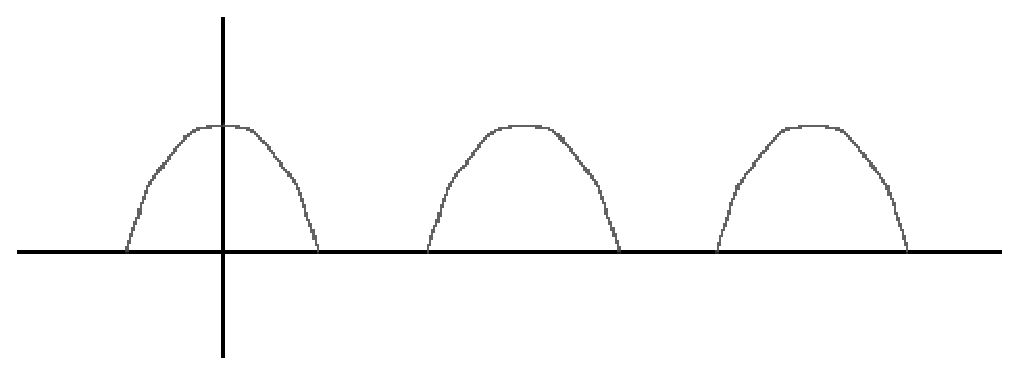
\includegraphics[width=0.8\linewidth,keepaspectratio]{fig/fig2_4.eps}
\caption{標本値のFourier変換。y軸のあたりに現れる原信号が、右側に等間隔で再度現れている}\label{fig2_4}
\end{figure}

このとき、同一のスペクトルの「ズレ」は$\frac{2\pi}{T}$という周波数になり、原信号のスペクトルの両裾とスペクトルの中心(0)間の距離は原信号の最大周波数に相当する。この裾同士が重なり合わないようにサンプリングできれば、1つの山=原信号だけを取り出すことができる。したがって、「ズレ」の間に原信号のスペクトル1つ分がすっぽり入れば良い。式でいうところでは、$\frac{2\pi}{T}$の間に原信号のスペクトル1つ分=最大周波数の2倍が入れば良いということになるので$\frac{2\pi}{T}$は最大周波数の2倍より大きければいいということになる。ここで、$\frac{2\pi}{T}$はサンプリング周期の逆数と$2\pi$をかけたものであるから、サンプリング周波数そのものである。

\section{標本値の量子化}
標本値を取得することで、アナログデータから離散値=デジタルデータを抜き出すことが出来た。しかし、これではまだ記録するには不十分である。というのは、標本値は必ずしも表現可能な数値とは限らないためである。

端的な例として、1辺が1の正方形の対角線の長さを考えよう。三平方の定理を鑑みればその長さが$\sqrt{2}$であることは明らかである。しかし、我々はこれを数値としてそのまま完全に保持することは出来ない。なんとならば、$\sqrt{2}$は無限に続く上に分数としても表現できない、無理数だからである。有限の10進値なり2進値なりで保持あるいは計算するというデジタルデータの原則に沿う限りにおいて、$\sqrt{2}$を保存するには無限の状態が必要となる。無論現実に無限の状態を用意できるわけもないため、必要な精度を以って我々はデータを丸める。つまり、切り捨てたり切り上げたりして表現可能にした近似値を$\sqrt{2}$の値として保存する。

実際には表現可能な数の一覧を尺度として準備しておき、このうち最も近い値として保存する。保存された値のことを量子化値と呼ぶ。量子化のレベル(尺度)は線形軸とする場合が多く、その幅こそ異なれど表現可能な数値の個数は変わらない。勿論、尺度を細かくするほど必要なデータも大きくなる。同じデータであっても線形$256$段階に分けるなら$8$ビットが必要となるが、これが線形$64$段階でいいなら$6$ビットで問題ない。この尺度はデータによって必要な精度等によって変わる。$n$ビットに量子化する場合、そのレベル値は$2^n$個になる。例えば、標本化の折に例を挙げたCD-DA規格は16bit=256レベルで、0dbから96dbまでの振幅を対象に量子化している。

まとめれば、量子化というのは、規格等によって用意された$2^n$個の尺度のうち最も近い値に標本値を丸める行為をいう。

\subsection{量子化雑音}
ここまで読んで明らかな通り標本値と量子化値には誤差が生じる。この誤差を\textbf{量子化雑音}\index{りょうしかざつおん@量子化雑音}と呼ぶ。アナログデータをデジタルデータに変換する際に量子化雑音は避けては通れない問題である。

量子化雑音がどれぐらいになるか見てみよう。最大値$H$、最小値$L$のデータを$n$ビットで量子化した場合、その各データの幅$D$は
\begin{equation}
D=\frac{|H-L|}{2^n-1}
\end{equation}
で与えられる(レベル値=目盛りが全部で$2^n$個あるため、その間を等分したもの)。今、最小値を基準にデータを表すとすれば、量子化値$Q$は
\begin{equation}
Q=L+Dk \ (k=0,1,\cdots,2^n-1)
\end{equation}
と記述できる。したがって標本値$S$との誤差は
\begin{equation}
|S-Q|=|S-(L+Dk)|
\end{equation}
となる。勿論、$k$は誤差が最小になるように選ばれる=標本値に近い側に丸められるのが普通であるので、これを仮定すると
\begin{equation}
|S-Q|=|S-(L+Dk)|\le \frac{D}{2}
\end{equation}
であることがわかる。

量子化雑音を小さくする、つまり標本値の再現精度を上げるためには当然ビット数を増やすことになる。しかし、量子化レベルを1bit増やすということは、全ての標本値を表すのに、各々1bitずつ増やして表現することとなるため、無闇に精度をあげるとデータが肥大化してしまう。このため、データの特性に応じて必要限度のbitを確保するのが一般的である。

\section{量子化値の符号化}
先の標本化・量子化を経てアナログデータをデジタルデータに変換できた。この後の保存は勿論先に学んだデジタルデータと同じように符号化して保存することとなる。

このとき、量子化値の性質によっては用いる符号を考慮して圧縮するなどの場合もある。ランレングスにより圧縮を書ける場合もあれば、連続である以上似たような値が続くと考えられることから差分を抽出し、これにエントロピー符号を適用するなどの手法が考えられる。

\section{値の復元}

逆に、符号化されたデータから原データを復元することを考える。基本的には、ここまでの手順を逆行するだけである。

最初に符号を読み取り、量子化値に戻す。これは実質的に(正しい手順で)符号を読むだけである。次に、量子化値を標本値として周波数スペクトルを求め(勿論、量子化値と標本値は別のものである。だが、量子化の手順で見たとおり、量子化値と標本値の差異は量子化雑音として捨てられたものであり、元の標本値をそのまま求めることは出来ない。そのため、量子化値=標本値の近似値を元の近似値として扱うのである。)、標本値以外の箇所における原データの値を計算する。その値を必要な形式で出力すれば、原データが復元できたと言えよう。

\section*{演習問題}
\begin{problems}
\item 光・音・運動の3データ以外の何らかのデータについて、デジタルへの変換なしに記録あるいは保存する方法を例示せよ。% 時計、熱電対、温度計等

\item 文中に出てきたCD-DAにおいては、44.1kHzのサンプリング周波数で16bit量子化している。また、ステレオ再生とするため、原データは2つに分かれており、その各々が先の通りサンプリングされている。
\begin{enumerate}
\item 1秒あたり何bitの容量が必要となるか(ビットレート)計算せよ。
\item 長さの異なるCD-DA音源のWaveファイルを4〜5個用意し、その再生時間(秒)と容量(ビット)のグラフを作成してみよ(圧縮されているWaveファイルもあるので、長さに対してあまりにサイズが小さい場合は除外すること)。また、そのグラフを直線で結んだときの傾き(ビットレート)と切片(Waveファイルのヘッダサイズ)を求めよ。(Waveファイルを作成する手っ取り早い方法として、適当なCDアルバム1枚をWaveファイルで取り込む方法を挙げておく。)
\end{enumerate}

\item 量子化雑音による誤差が最大0.05℃に収まるように、気温のデータをサンプリングしたい。期待されるデータの最高気温が60℃、最低気温が-90℃であるとき、量子化値の表現には何bitが必要となるか。
\end{problems}
